\documentclass{beamer}
\usepackage[utf8]{inputenc}
\usetheme{Antibes}
\usecolortheme{beaver}
\usepackage{parskip}
\usepackage{graphicx}
\usepackage{hyperref}
\urlstyle{same}

\title{Tuning, Temperament, Timbre, and Twos}
\subtitle{Why Rectifying Resonant Ratios Requires Roots}
\author{Jesse He}
\institute{OSU Reading Classics}
\date{October 6, 2020}

\begin{document}

\frame{\titlepage}

\section{The Greeks}
\subsection{Pythagoras, Strings, and the Square Root of Two}
\begin{frame}{Pythagoras, Strings, and the Square Root of Two}
    \pause Pythagoras of Samos (c.570-c.495 BCE) is credited as the first to describe music mathematically.
    
    \pause The Pythagoreans noticed that a taught string of a particular length would sound consonant when plucked with a string half the length of the first.
    
    \pause This became the basis for the octave, which is the basis for most musical scales across different cultures.
\end{frame}

\begin{frame}{Pythagoras, Strings, and the Square Root of Two}
    \pause The \textit{Manual of Harmonics} (\textit{Encheiridion Harmonikes}) by Nicomachus of Gerasa (60-c.120 AD) contains the legend of the Pythagorean hammers.
    
    \pause Allegedly, Pythagoras noticed while listening to the sound of four blacksmiths' hammers that some hammers would sound consonant when struck together, while others would sound dissonant.
    
    \pause Upon examining the hammers, Pythagoras found that hammers whose weights were simple integer ratios would sound consonant while those which were not sounded dissonant.
    
    \pause This legend is demonstrably false.
\end{frame}

\begin{frame}{Pythagoras, Strings, and the Square Root of Two}
    \pause The Pythagoreans thought that integer ratios should be the basis for their music, which led to their development of the harmonic mean:
    \pause
    \[
        HM(x_1, \dots, x_n) = \dfrac{n}{\sum_{i=1}^n \frac{1}{x_i}}
    \]
    \pause Because of their obsession with integer ratios, the Pythagoreans were allegedly rather displeased to find, for example, that $\sqrt{2}$ is not rational.
\end{frame}

\subsection{Ptolemy's Intense Diatonic Scale}
\begin{frame}{Ptolemy's Intense Diatonic Scale}
    \pause Claudius Ptolemy (c.100-c.170 CE), in \textit{Harmonics}, described the intense (or syntonic) diatonic scale, which became the basis for the modern Western major scale.
\end{frame}

\section{Harmonics}
\subsection{Why Integer Ratios?}
\begin{frame}{Why Integer Ratios?}
    \pause The reason integer ratios produce the consonance Pythagoras observed is physical.
    
    \pause When a string (or other sound-making object) vibrates at a frequency $f$, it also produces vibrations at integer multiples of $f$.
    \pause We call $f$ the fundamental and these other vibrations \textit{harmonics} (or overtones), which produce the harmonic series:
    \pause $$ \sum_{n=1}^\infty \frac{1}{n} $$
\end{frame}
\begin{frame}{Why Integer Ratios?}
    \begin{minipage}{.49\textwidth}
        \pause Because the length of a string is fixed, the harmonics must have fixed points at either end.
        
        \pause As a result, the frequency of a harmonic must be an integer multiple of the fundamental $f$.
        
        \pause Because the frequency is inversely proportional to period, the period of each harmonic is some fraction of $f$.
    \end{minipage}
    \begin{minipage}{.49\textwidth}
        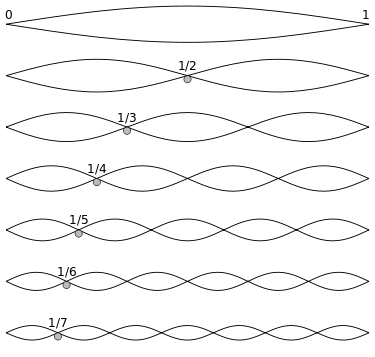
\includegraphics[width=\textwidth]{harmonic-series.png}
    \end{minipage}
\end{frame}

\subsection{Timbre and Fourier Analysis}
\begin{frame}{Timbre and Fourier Analysis}
    \pause The exact amplitude of the harmonics produced by a sound differ based on different physical constraints.
    
    \pause These subtle differences in overtones create different sounds, which musicians refer to as \textit{timbre}.
    
    \pause We can, however, use the machinery of Fourier analysis to decompose a sound into its component wavelengths!
\end{frame}

\begin{frame}{Timbre and Fourier Analysis}
    $$y \approx  2.189\sin(x)$$
    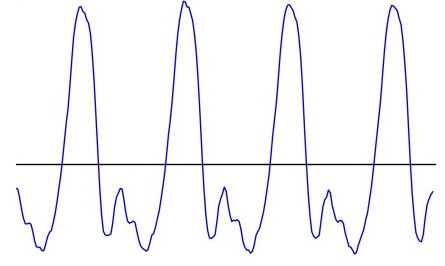
\includegraphics[width=.49\textwidth]{violin_waveform.jpg}
    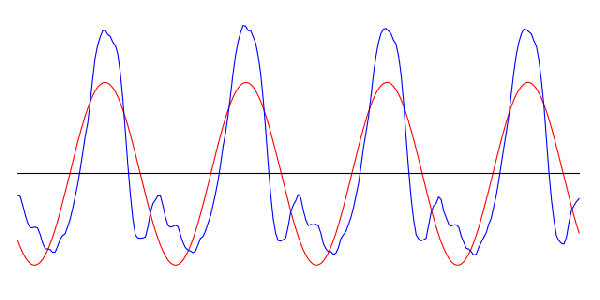
\includegraphics[width=.49\textwidth]{Violin_Fourier_Frames/frame_1_delay-1s.png}
\end{frame}

\begin{frame}{Timbre and Fourier Analysis}
    $$y \approx  2.189\sin(x) + 1.256\sin(2x)$$
    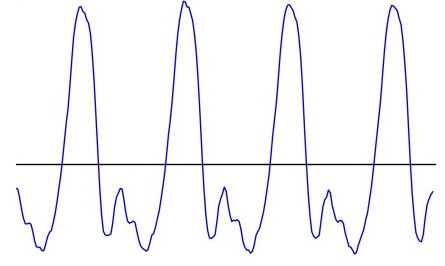
\includegraphics[width=.49\textwidth]{violin_waveform.jpg}
    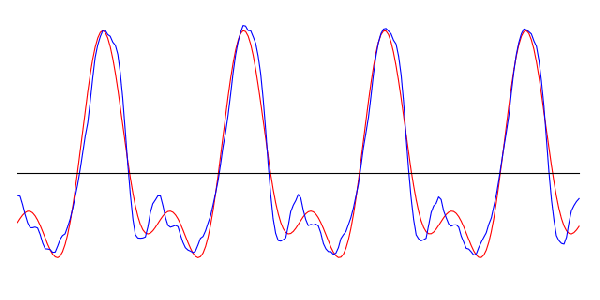
\includegraphics[width=.49\textwidth]{Violin_Fourier_Frames/frame_2_delay-1s.png}
\end{frame}

\begin{frame}{Timbre and Fourier Analysis}
    $$y \approx  2.189\sin(x) + 1.256\sin(2x) + 0.459\sin(3x)$$
    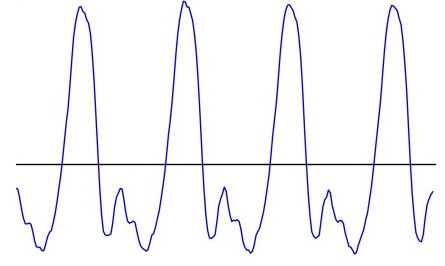
\includegraphics[width=.49\textwidth]{violin_waveform.jpg}
    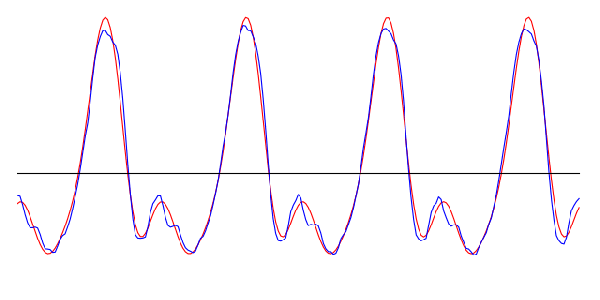
\includegraphics[width=.49\textwidth]{Violin_Fourier_Frames/frame_3_delay-1s.png}
    \tiny{Oh? You're approaching me?}
\end{frame}

\begin{frame}{Timbre and Fourier Analysis}
    $$y \approx  2.189\sin(x) + 1.256\sin(2x) + 0.459\sin(3x) + 0.182\sin(4x)$$
    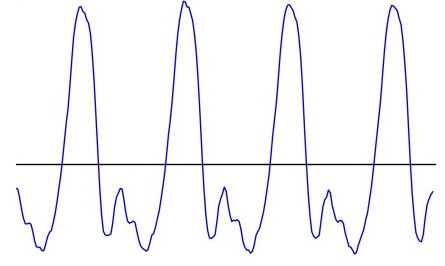
\includegraphics[width=.49\textwidth]{violin_waveform.jpg}
    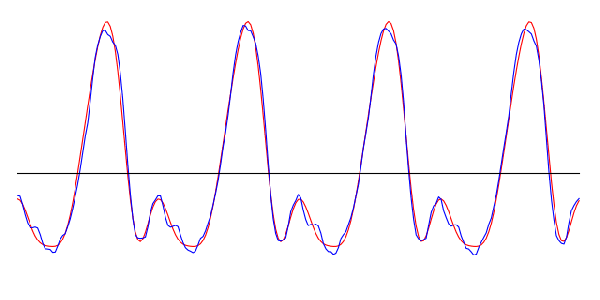
\includegraphics[width=.49\textwidth]{Violin_Fourier_Frames/frame_4_delay-1s.png}
\end{frame}

\section{Just Intonation}
\subsection{Classical Just Intonation}
\begin{frame}{Classical Just Intonation}
    \pause Ptolemy's intense diatonic scale can be extended to the  twelve notes of the modern (chromatic) scale.
    
    \pause By defining each note by an integer ratio of a fixed frequency, we can guarantee the consonance that Pythagoras and Ptolemy observed.
\end{frame}

\subsection{Pythagorean Tuning}
\begin{frame}{Pythagorean Tuning}
    \pause Another way to define the scale is to define notes by powers of one or two specific ratios.
    
    \pause This gives rise to \textit{syntonic temperament}. If we base our scale around powers of $2$ and $\frac{3}{2}$, we get Pythagorean tuning (also known as 3-limit just intonation).
\end{frame}

\subsection{Wolf Intervals}
\begin{frame}{Wolf Intervals}
    \pause The ``bad'' intervals in these scales are known as wolf intervals.
    
    \pause As an example, we will work out the interval between F$\sharp$ and C$\sharp$ in Pythagorean tuning, which we expect to be $\frac{3}{2}$:
\end{frame}

\begin{frame}{Wolf Intervals}
    \pause We will do our calculations with respect to the note C, whose ratio to itself is of course 1. Since Pythagorean tuning is based on $\frac{3}{2}$ (in music, a perfect fifth), we will use the circle of fifths:
    
    \begin{minipage}{.49\textwidth}
        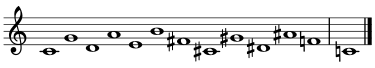
\includegraphics[width=\textwidth]{citcle-of-fifths.png}
    \end{minipage}
    \begin{minipage}{.49\textwidth}
        \small{C-G-D-A-E-B-F$\sharp$-C$\sharp$-G$\sharp$-D$\sharp$-A$\sharp$-F-C}
    \end{minipage}
    
    \pause Since F$\sharp$ is 6 fifths above C, its ratio to C is
    $\left( \frac{3}{2} \right)^6$. To normalize the octave, we divide by 2 three times to get $\left( \frac{3}{2} \right)^6 \left( \frac{1}{2} \right)^{3}$
    
    \pause To get to C$\sharp$ we continue along the circle of fifths and multiply by $\frac{3}{2}$, right?
    
    \pause Well, we can also move backwards: C$\sharp$ is 5 fifths \textit{below} C, so after normalizing octaves, we get that it should be $\left( \frac{2}{3} \right)^5 2^4$
\end{frame}

\begin{frame}{Wolf Intervals}
    So we end up with two possible values for C$\sharp$: $\left( \frac{3}{2} \right)^7 \left( \frac{1}{2} \right)^{3}$ or $\left( \frac{2}{3} \right)^5 2^4$. (The difference between these is known as the Pythagorean comma).
    
    \pause Since $\left( \frac{2}{3} \right)^5 2^4$ has a lower exponent, it is in some sense the ``simpler'' ratio, so we should take that one to define C$\sharp$.
    
    \pause But then the ratio between F$\sharp$ and C$\sharp$ is
    \[
        \frac{\left( \frac{3}{2} \right)^6 \left( \frac{1}{2} \right)^{3}}{\left( \frac{2}{3} \right)^5 2^4}
        = \frac{2^9 3^{-5}}{3^6 2^{-9}}
        = \frac{2^{18}}{3^{11}}
        = \frac{262144}{177141}
        \approx 1.47981
        \neq \frac{3}{2}
    \]
    
    \pause This is not a simple integer ratio.
\end{frame}

\begin{frame}{Wolf Intervals}
    \pause Classical just intonation is even worse: the same interval (F$\sharp$ to C$\sharp$) is a wolf interval of $\frac{32}{21}$, but the interval D to A is another wolf interval of $\frac{40}{27}$.
    
    \pause So even though the ratios look simpler, inside this scale there are two wolves!
\end{frame}

\begin{frame}{The Devil in Music}
    \pause Because F$\sharp$ is halfway between the root (C) and the octave, is is particularly difficult to assign an integer ratio to it in any system.
    
    \pause The interval between C and F$\sharp$ is particularly dissonant, earning it the historical nickname ``Diabolus in Musica'' (the Devil in Music).
\end{frame}

\subsection{Benedetti's Puzzle}
\begin{frame}{Benedetti's Puzzle}
    \pause Another consequence of just intonation is the ``comma pump,'' as described by Italian mathematician Gianbattista Benedetti (1530-1590).
    
    \pause In a letter to Italian composer Cipriano de Rore, Benedetti described the phenomenon of singers in a choir slowly drifting in pitch, away from where they began singing a piece.
    
    \pause This is known as a \textit{comma pump}.
\end{frame}

\begin{frame}{Benedetti's Puzzle}
    \begin{tabular}{r|l}
        Octave & 2 \\
        Fifth & $\frac{3}{2}$ \\
        Major Third & $\frac{5}{4}$
    \end{tabular}
    \hspace{1cm}
    \begin{tabular}{cccc}
        G & A & - & G \\
        D & - & E & - \\
        G & - & C & -
    \end{tabular}
    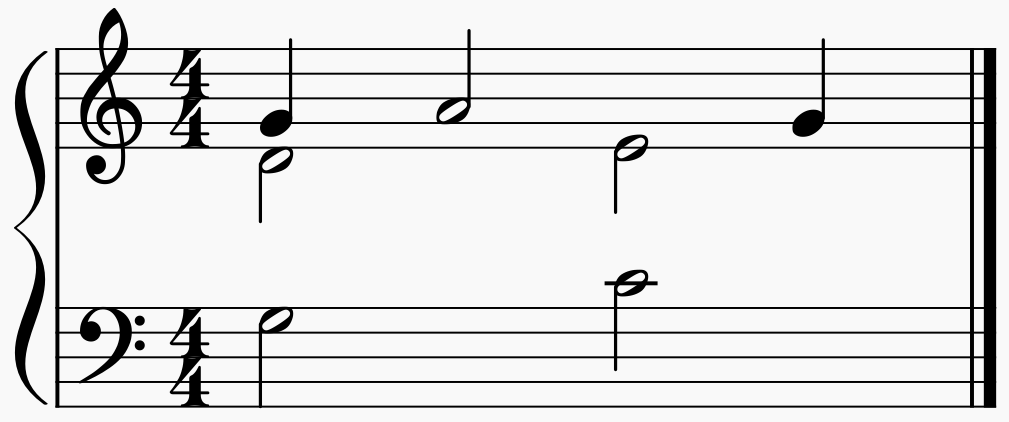
\includegraphics[width=\textwidth]{benedetti-puzzle.png}
\end{frame}

\section{Equal Temperament}
\subsection{Taming the Wolf}
\begin{frame}{Taming the Wolf}
    \pause The goal of many musicians throughout the Renaissance and Baroque eras was to eliminate wolf tones and comma pumps through some new tuning system.
    
    \pause ``We are compell’d to use an occult Temperament, and to sing these imperfect Intervals, from doing which less offence arises.''
    
    \pause To paraphrase, ``I, Gianbattista Benedetti, have a dream...''
\end{frame}

\begin{frame}{Taming the Wolf}
    \pause The new tuning systems proposed included meantone and well-temperament (the latter being the basis of Johann Sebastian Bach's famous composition ``The Well-Tempered Clavier'' in 1722).
    
    \pause The idea was to distort a few intervals in order to spread any discrepancy across several intervals.
\end{frame}

\subsection{Zhu Zaiyu}
\begin{frame}{Zhu Zaiyu's Pitch Pipes}
    \pause The first to formulate and precisely calculate an \textit{equal-tempered} system was Chinese mathematician, musician, and choreographer Zhu Zaiyu (1536-1611).
    
    \pause Zhu developed a twelve-tone equal temperament based on the twelfth root of 2 in 1584:
\end{frame}

\begin{frame}{Zhu Zaiyu's Pitch Pipes}
    \begin{minipage}{.49\textwidth}
        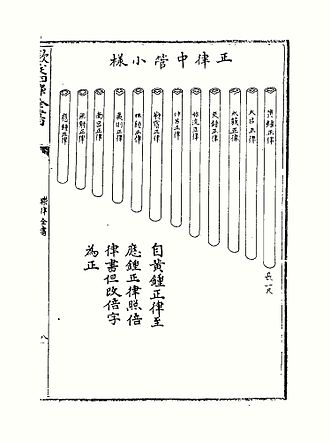
\includegraphics[width=\textwidth]{zhu-zaiyu-pipes.jpg}
    \end{minipage}
    \begin{minipage}{.49\textwidth}
        ``I have founded a new system. I establish one foot as the number from which the others are to be extracted, and using proportions I extract them. Altogether one has to find the exact figures for the pitch-pipers in twelve operations.''
    \end{minipage}
\end{frame}

\subsection{The Twelfth Root of Two}
\begin{frame}{The Twelfth Root of Two}
    \pause Zhu Zaiyu's equal temperament was independently invented by Simon Stevin in 1585, whose calculations were later refined by Martin Mersenne and then by Johann Faulhaber in 1630.
    
    \pause Using the twelth root of two intuitively makes sense: we want to divide the octave (whose frequency is twice the fundamental's) into twelve equal parts, so $\sqrt[12]{2}$ should be the basis of our division.
\end{frame}

\section{Conclusion}
\begin{frame}{Full (Tone) Circle}
    \pause Using roots of two also generalizes very well to other scales: simply use the $n$-th root of 2 to divide the octave into $n$ evenly spaced notes.
    
    \pause When we write out the ratios of this ``occult temperament,'' as Benedetti wrote, we see a familiar figure...
    
    \pause 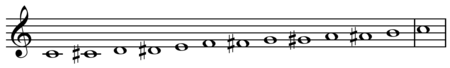
\includegraphics[width=\textwidth]{12-tone-scale.png}
    \begin{table}
        \centering
        \begin{tabular}{cccccccccccc|c}\small
            C & C$\sharp$ & D & D$\sharp$ & E & F & F$\sharp$ & G & G$\sharp$ & A & A$\sharp$ & B & C \\
            1 & $2^{\frac{1}{12}}$ & $2^{\frac{1}{6}}$ & $2^{\frac{1}{4}}$ & $2^{\frac{1}{3}}$ & $2^{\frac{5}{12}}$ & $2^{\frac{1}{2}}$ & $2^{\frac{7}{12}}$ & $2^{\frac{2}{3}}$ & $2^{\frac{3}{4}}$ & $2^{\frac{5}{6}}$ & $2^{\frac{11}{12}}$ & 2
        \end{tabular}
    \end{table}
\end{frame}

\section{References}
\begin{frame}{References}
    \footnotesize
    Christensen, Thomas, editor. \textit{The Cambridge History of Western Music Theory}. Cambridge University Press, 2002.  doi:10.1017/CHOL9780521623711
    
    Duffin, Ross. ``Just Intonation in Renaissance Theory \& Practice". College of Arts and Sciences, Case Western Reserve University, 2017. https://casfaculty.case.edu/ross-duffin/just-intonation-in-renaissance-theory-practice/
    
    Johnston, Ben and Bob Gilmore. ``MAXIMUM CLARITY" AND OTHER WRITINGS ON MUSIC. University of Illinois Press, 2006. Project MUSE muse.jhu.edu/book/18567.
    
    ``The Fourier Transform and the Spectrum", Tremblings and Warblings, 2017. http://www.tremblingsandwarblings.com/2017/05/fourier-transform-spectrum/
    
    Wikipedia, Intern \textit{et al.}
\end{frame}

\end{document}
